\documentclass[landscape]{article}
\usepackage{tikz}
\usetikzlibrary{shapes,arrows,positioning}
\usepackage{geometry}

% Adjust the page layout with the geometry package
\geometry{left=2cm, right=2cm, top=2cm, bottom=2cm}

\begin{document}
\begin{figure}
    \centering
    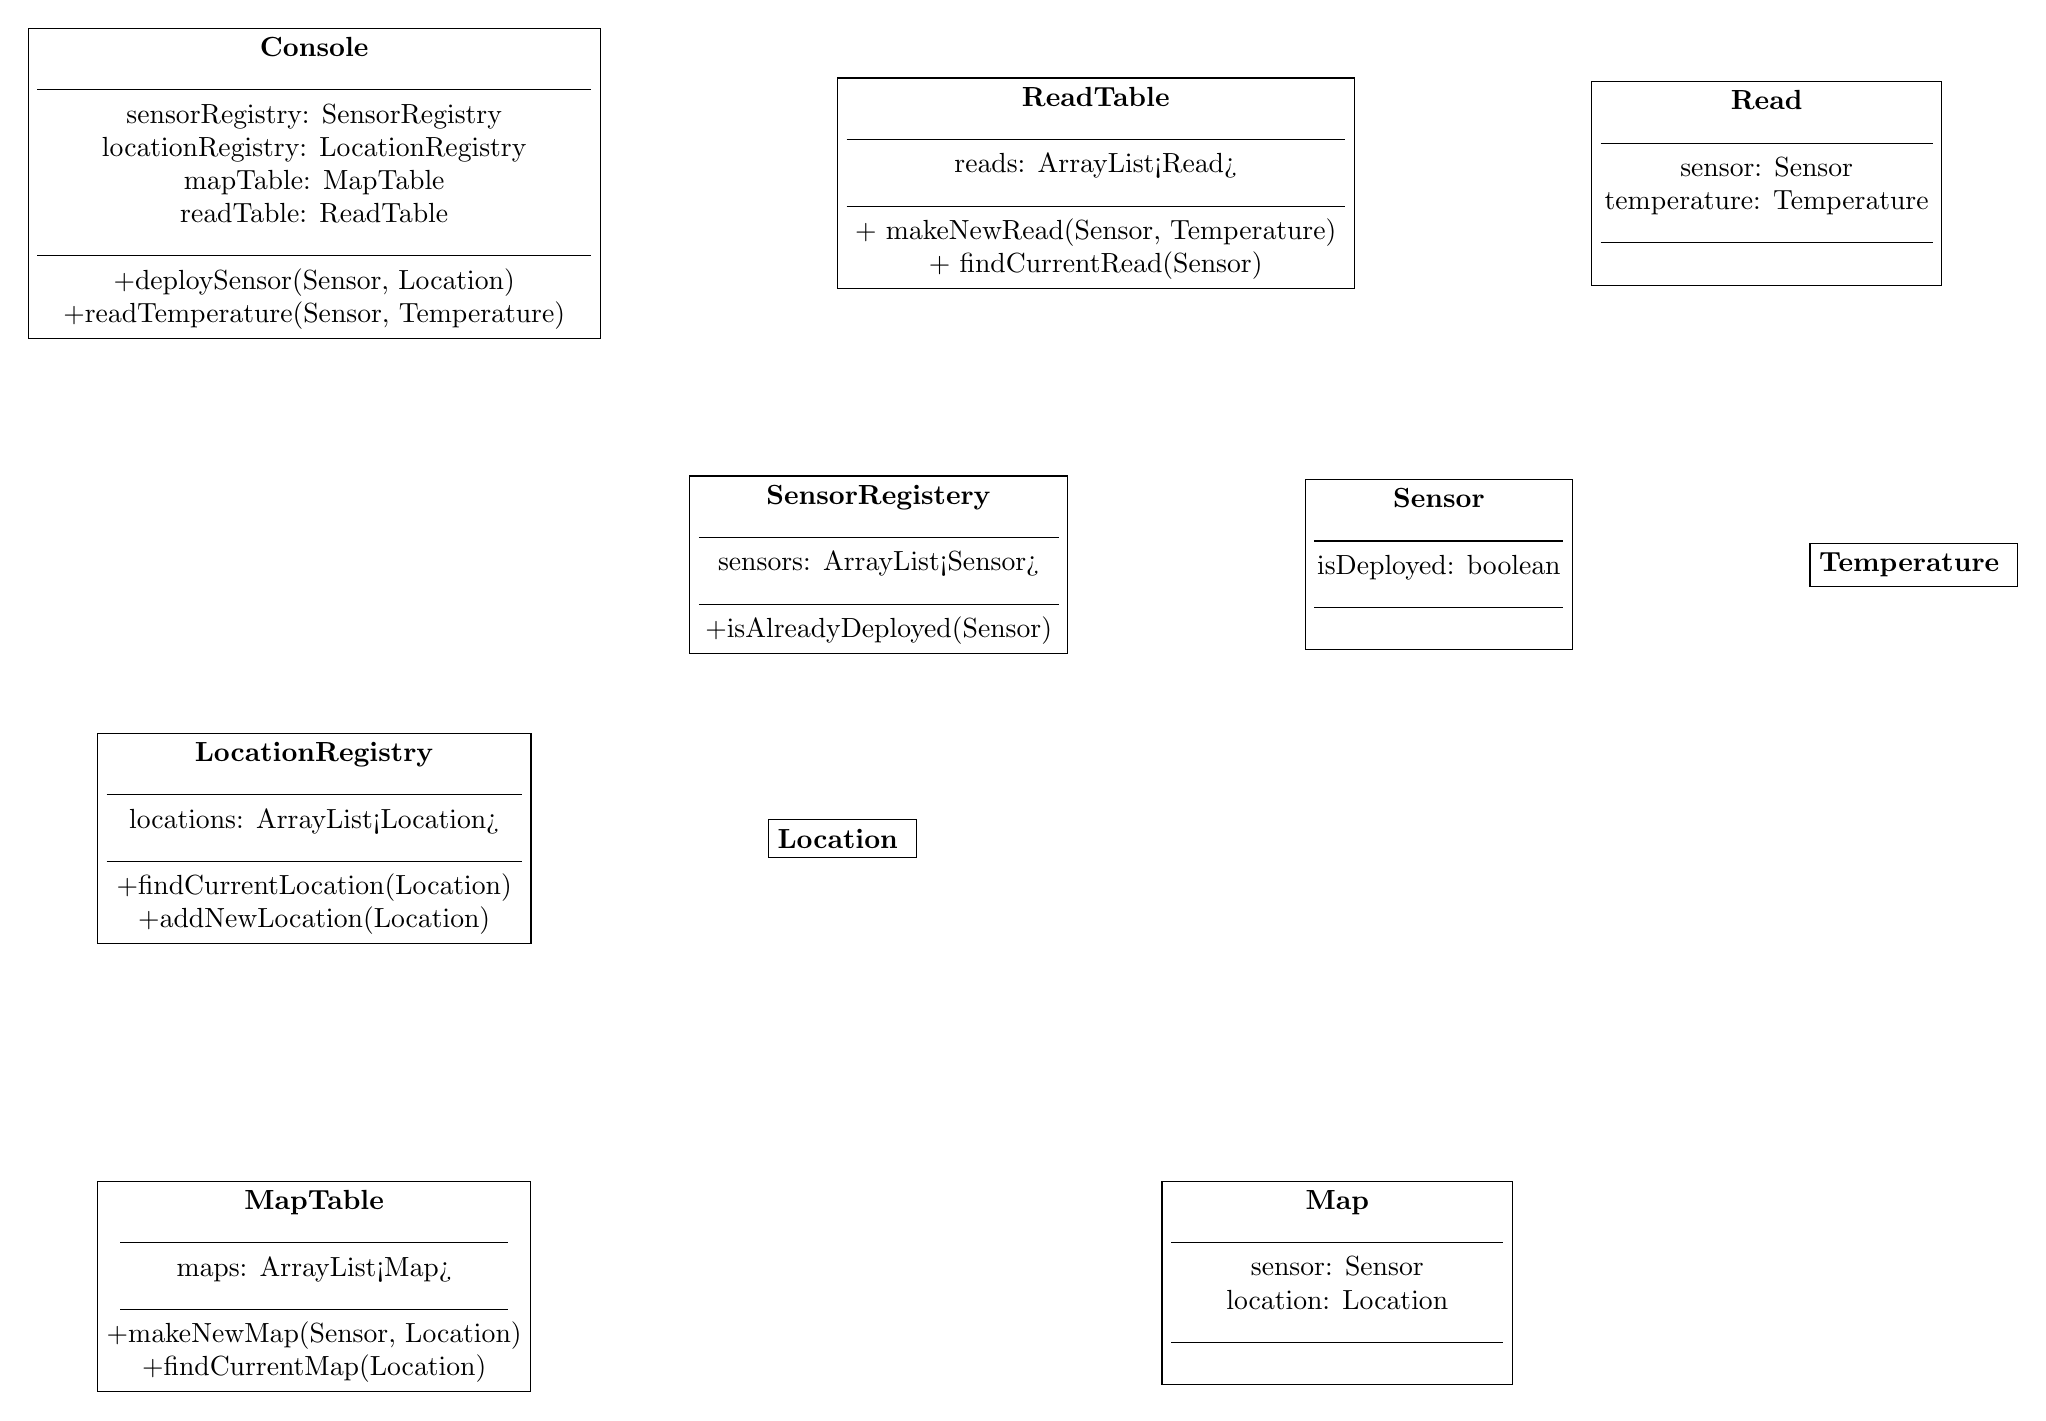
\begin{tikzpicture}
    
    	%-----Classes-----
        % Console Class
        \node [rectangle, draw, align=center] (console) {%
            \textbf{Console} \\
            \line(1,0){200} \\
            sensorRegistry: SensorRegistry \\
            locationRegistry: LocationRegistry \\
            mapTable: MapTable \\
            readTable: ReadTable \\
            \line(1,0){200} \\
            +deploySensor(Sensor, Location) \\
            +readTemperature(Sensor, Temperature)
        };
        
        % Location Registry Class
        \node [rectangle, draw, below=5cm of console, align=center] (lreg) {%
            \textbf{LocationRegistry} \\
            \line(1,0){150} \\
            locations: ArrayList<Location> \\
            \line(1,0){150} \\
            +findCurrentLocation(Location) \\
            +addNewLocation(Location)
        };
        
        % Read Table Class
        \node [rectangle, draw, right=3cm of console, align=center] (readt) {%
            \textbf{ReadTable} \\
            \line(1,0){180} \\
            reads: ArrayList<Read> \\
            \line(1,0){180} \\
            + makeNewRead(Sensor, Temperature) \\
            + findCurrentRead(Sensor)
        };
		
		 % Read Class
        \node [rectangle, draw, right=3cm of readt, align=center] (read) {%
            \textbf{Read} \\
            \line(1,0){120} \\
            sensor: Sensor \\
            temperature: Temperature \\
            \line(1,0){120} \\
        };
        
         % Sensor Registry Class
        \node [rectangle, draw, above right=1cm and 2cm of lreg, align=center] (sreg) {%
            \textbf{SensorRegistery}\\
            \line(1,0){130} \\
            sensors: ArrayList<Sensor> \\
            \line(1,0){130} \\
            +isAlreadyDeployed(Sensor)
        }; 
        
        % Sensor Class
        \node [rectangle, draw, right=3cm of sreg, align=center] (sensor) {%
            \textbf{Sensor} \\
            \line(1,0){90} \\
            isDeployed: boolean \\
            \line(1,0){90} \\
        };
       
       % Temperature Class
        \node [rectangle, draw, right=3cm of sensor, align=center] (temp) {%
            \textbf{Temperature} 
        };
        
        % Location Class
        \node [rectangle, draw, right=3cm of lreg, align=center] (loc) {%
            \textbf{Location} 
        };
        
        % Location Map Class
        %\node [rectangle, draw, below=2cm of loc, align=center] (locmap) {%
            %\textbf{LocationMap} 
        %};
        
        % Map Table Class
        \node [rectangle, draw, below=3cm of lreg, align=center] (mapt) {%
            \textbf{MapTable}  \\
            \line(1,0){140} \\
            maps: ArrayList<Map> \\
            \line(1,0){140} \\
            +makeNewMap(Sensor, Location) \\
            +findCurrentMap(Location)
        };
        
         % Map Class
        \node [rectangle, draw, below right=3cm and 8cm of lreg, align=center] (map) {%
            \textbf{Map}  \\
            \line(1,0){120} \\
            sensor: Sensor \\
            location: Location \\
            \line(1,0){120} \\
        };
        
        
    \end{tikzpicture}
    \caption{UML Class Diagram for Sensor System}
\end{figure}
\end{document}
